\documentclass{article}
\usepackage{amsmath,amssymb}
\usepackage{graphicx}
\usepackage{enumerate}
\usepackage{hyperref}
\usepackage{subcaption}
\usepackage{caption}
\usepackage{xcolor}
\usepackage{float}

\pagestyle{empty} \addtolength{\textwidth}{1.0in}
\addtolength{\textheight}{0.5in}
\addtolength{\oddsidemargin}{-0.5in}
\addtolength{\evensidemargin}{-0.5in}
\newcommand{\ruleskip}{\bigskip\hrule\bigskip}
\newcommand{\nodify}[1]{{\sc #1}}
\newcommand{\points}[1]{{\textbf{[#1 points]}}}
\newcommand{\subquestionpoints}[1]{{[#1 points]}}
\newenvironment{answer}{{\bf Answer:} \sf }{}%

\newcommand{\bitem}{\begin{list}{$\bullet$}%
{\setlength{\itemsep}{0pt}\setlength{\topsep}{0pt}%
\setlength{\rightmargin}{0pt}}}
\newcommand{\eitem}{\end{list}}

\setlength{\parindent}{0pt} \setlength{\parskip}{0.5ex}
\setlength{\unitlength}{1cm}

\newcommand{\pa}[1]{[[PA: #1]]}

\renewcommand{\Re}{{\mathbb R}}
\newcommand{\E}{{\rm E}}
\begin{document}

\pagestyle{myheadings} \markboth{}{CS 294-158 Deep Unsupervised Learning, Homework 3, Spring 2024}

{\huge
\noindent Homework 3: GAN Models}
\ruleskip

{\bf Deliverable}: This PDF write-up by {\bf Tuesday March 6th, 23:59pm}.  Your PDF should be generated by simply replacing the placeholder images of this LaTeX document with the appropriate solution images that will be generated automatically when solving each question. The solution images are automatically generated and saved using the accompanying IPython notebook. Your PDF is to be submitted into Gradescope. This PDF already contains a few solution images.  These images will allow you to check your own solution to ensure correctness.


\vspace{.2in}

%--------------------------------------------------------------------------------
%--------------------------------------------------------------------------------
%--------------------------------------------------------------------------------
\noindent {\bf Question 1: 1D Data}
%--------------------------------------------------------------------------------
%--------------------------------------------------------------------------------
%--------------------------------------------------------------------------------

\begin{enumerate}[(a)]

\item {\bf [10pt] Minimax GAN Objective} \\\\
\begin{figure}[H]
    \centering
    \begin{subfigure}{0.45\textwidth}
        \centering
        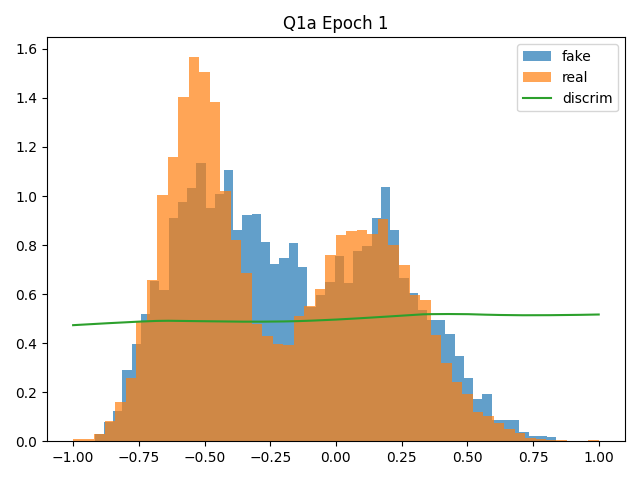
\includegraphics[width=\textwidth]{figures/q1a_epoch1.png}
        \caption{Samples at epoch 1}
    \end{subfigure}
    \begin{subfigure}{0.45\textwidth}
        \centering
        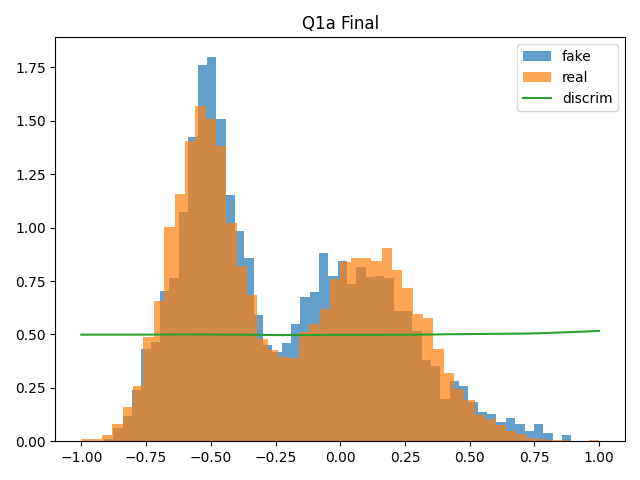
\includegraphics[width=\textwidth]{figures/q1a_final.png}
        \caption{Final samples}
    \end{subfigure}
    \\
    \begin{subfigure}{0.34\textwidth}
        \centering
        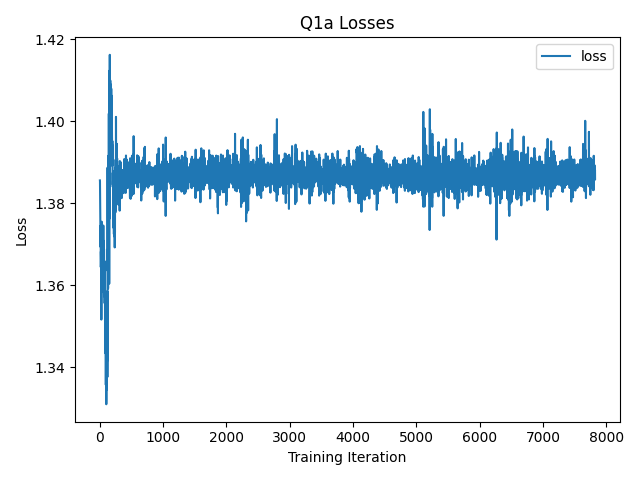
\includegraphics[width=\textwidth]{figures/q1a_losses.png}
        \caption{GAN loss curve}
    \end{subfigure}
\end{figure}
\newpage

\item {\bf [10pt] Nonsaturating Objective} \\\\
\begin{figure}[H]
    \centering
    \begin{subfigure}{0.45\textwidth}
        \centering
        
\includegraphics[width=\textwidth]{figures/q1b_epoch1.png}
        \caption{Samples at epoch 1}
    \end{subfigure}
    \begin{subfigure}{0.45\textwidth}
        \centering
        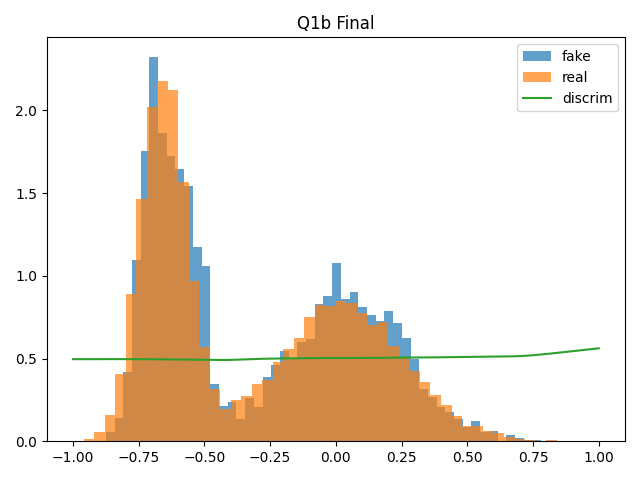
\includegraphics[width=\textwidth]{figures/q1b_final.png}
        \caption{Final samples}
    \end{subfigure}
    \\
    \begin{subfigure}{0.34\textwidth}
        \centering
        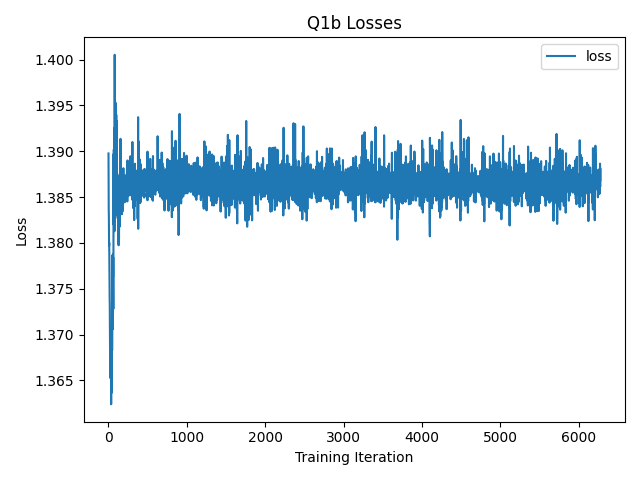
\includegraphics[width=\textwidth]{figures/q1b_losses.png}
        \caption{GAN loss curve}
    \end{subfigure}
\end{figure}
\end{enumerate}



%--------------------------------------------------------------------------------
%--------------------------------------------------------------------------------
%--------------------------------------------------------------------------------
\newpage
\noindent {\bf Question 2: WGAN-GP on CIFAR-10 [35pt]}
%--------------------------------------------------------------------------------
%--------------------------------------------------------------------------------
%--------------------------------------------------------------------------------



Final inception score: \textbf{7.933057} \\
Final Fréchet inception distance: \textbf{TODO}
\begin{figure}[H]
    \centering
    \begin{subfigure}{0.6\textwidth}
        \centering
        
\includegraphics[width=\textwidth]{figures/q2_samples.png}
        \caption{Samples}
    \end{subfigure}
    \\
    \begin{subfigure}{0.6\textwidth}
        \centering
        
\includegraphics[width=\textwidth]{figures/q2_losses.png}
        \caption{Training curve}
    \end{subfigure}

\end{figure}


%--------------------------------------------------------------------------------
%--------------------------------------------------------------------------------
%--------------------------------------------------------------------------------
\newpage
\noindent {\bf Question 3: Quantization with GANS [40 pt]}\\
%--------------------------------------------------------------------------------
%--------------------------------------------------------------------------------
%--------------------------------------------------------------------------------

\noindent {\bf Part a: Vanilla VQGAN [25 pt]}
Final l2 validation reconstruction loss: \textbf{0.03634011661633849} \\
\begin{figure}[H]
    \centering
    \begin{subfigure}{0.45\textwidth}
        \centering
        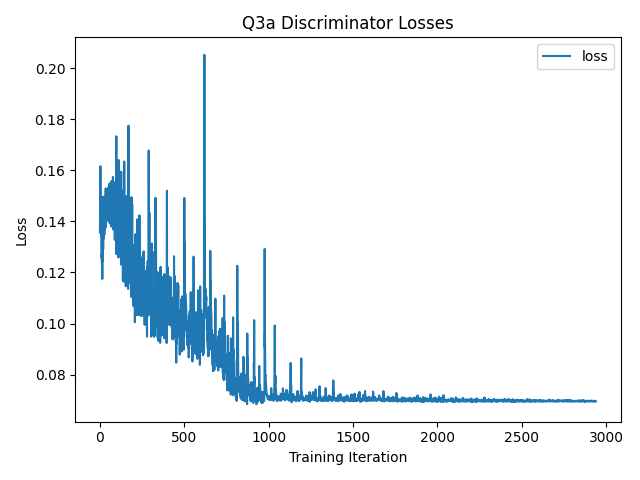
\includegraphics[width=\textwidth]{figures/q3a_gan_losses.png}
        \caption{Discriminator losses}
    \end{subfigure}
    \begin{subfigure}{0.45\textwidth}
        \centering
        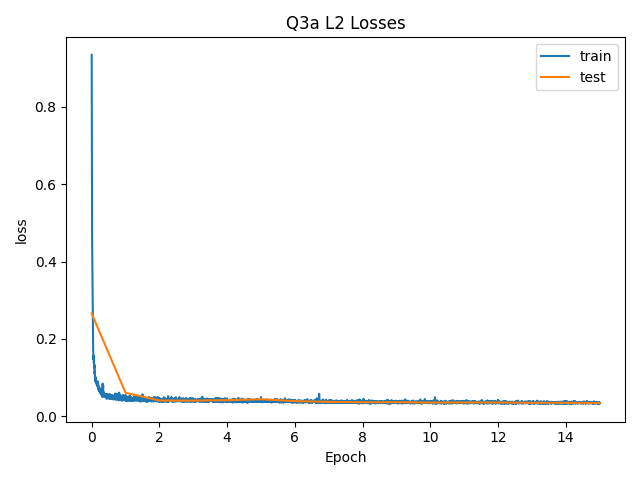
\includegraphics[width=\textwidth]{figures/q3a_l2_losses.png}
        \caption{L2 losses}
    \end{subfigure}
    \\
    \begin{subfigure}{0.4\textwidth}
        \centering
        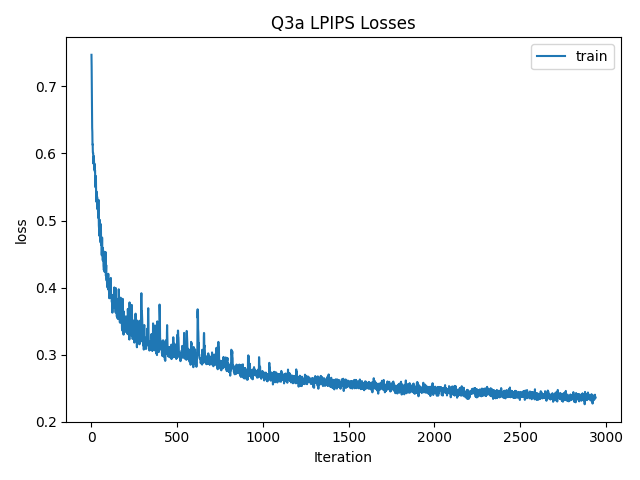
\includegraphics[width=\textwidth]{figures/q3a_lpips_losses.png}
        \caption{LPIPS losses}
    \end{subfigure}
    \begin{subfigure}{0.6\textwidth}
        \centering
        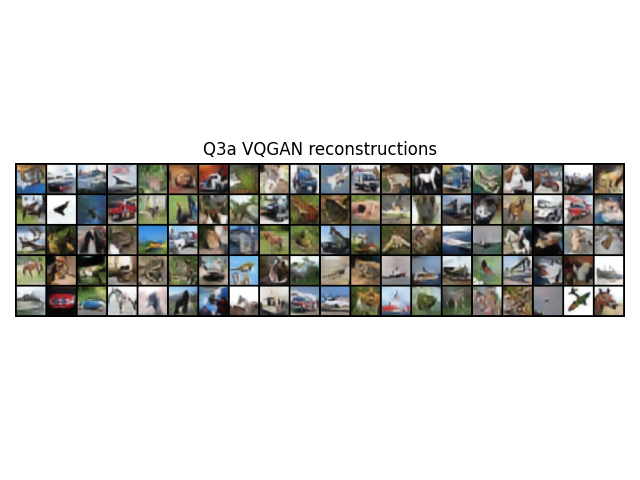
\includegraphics[width=\textwidth]{figures/q3a_reconstructions.png}
        \caption{Reconstructions}
    \end{subfigure}
\end{figure}

\noindent {\bf Part b: ViT-VQGAN [15 pt]}
% Slurm: homeworks/hw3/slurm/deepul.148575.out
Final l2 validation reconstruction loss: \textbf{0.06677825003862381} \\
\begin{figure}[H]
    \centering
    \begin{subfigure}{0.45\textwidth}
        \centering
        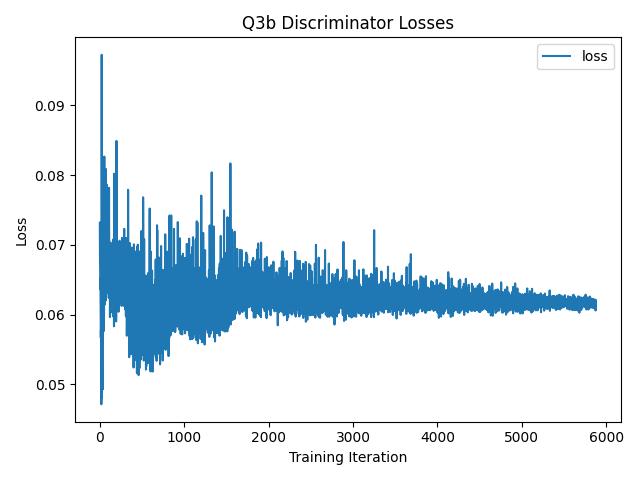
\includegraphics[width=\textwidth]{figures/q3b_gan_losses.png}
        \caption{Discriminator losses}
    \end{subfigure}
    \begin{subfigure}{0.45\textwidth}
        \centering
        
\includegraphics[width=\textwidth]{figures/q3b_l2_losses.png}
        \caption{L2 losses}
    \end{subfigure}
    \\
    \begin{subfigure}{0.4\textwidth}
        \centering
        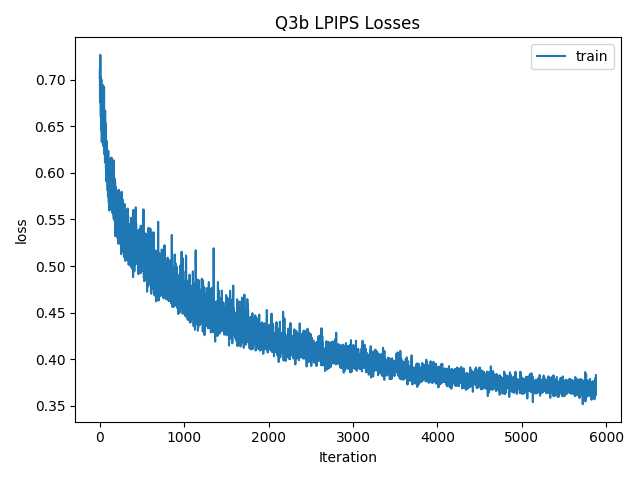
\includegraphics[width=\textwidth]{figures/q3b_lpips_losses.png}
        \caption{LPIPS losses}
    \end{subfigure}
    \begin{subfigure}{0.6\textwidth}
        \centering
        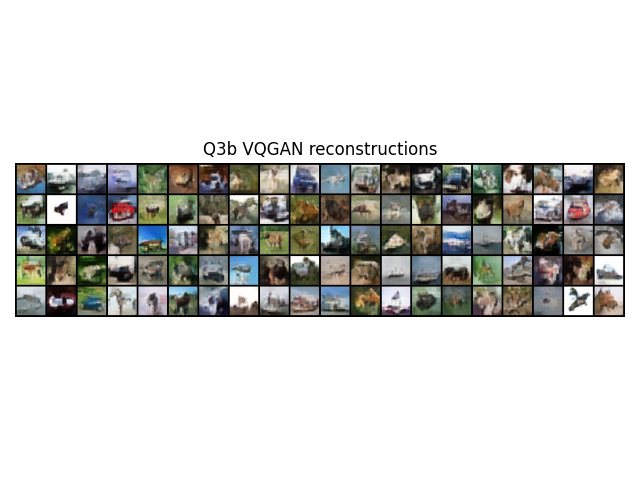
\includegraphics[width=\textwidth]{figures/q3b_reconstructions.png}
        \caption{Reconstructions}
    \end{subfigure}
\end{figure}

%--------------------------------------------------------------------------------
%--------------------------------------------------------------------------------
%--------------------------------------------------------------------------------
\newpage
\noindent {\bf Bonus Questions (Optional)}
%--------------------------------------------------------------------------------
%--------------------------------------------------------------------------------
%--------------------------------------------------------------------------------
\begin{enumerate}

\item {\bf [20pt] CycleGAN} \\\\
\begin{figure}[H]
    \centering
    \begin{subfigure}{0.5\textwidth}
        \centering
        \includegraphics[width=\textwidth]{figures/q4_mnist.png}
        \caption{MNIST: original images, translations, and reconstructions}
    \end{subfigure}
    \\
    \begin{subfigure}{0.5\textwidth}
        \centering
        \includegraphics[width=\textwidth]{figures/q4_colored_mnist.png}
        \caption{Colored MNIST: original images, translations, and reconstructions}
    \end{subfigure}
\end{figure}
\end{enumerate}

\end{document}
